\documentclass[11pt,xcolor=pdflatex,hyperref={unicode}]{beamer}
\usepackage{minted}
\usepackage{newcent}
\usepackage[utf8]{inputenc}
\usepackage[czech]{babel}
\usepackage[T1]{fontenc}
\usepackage{hyperref}
\usepackage{fancyvrb}
\usepackage{graphics}
\graphicspath{ {./img/} }
\usetheme{FIT}

%%%%%%%%%%%%%%%%%%%%%%%%%%%%%%%%%%%%%%%%%%%%%%%%%%%%%%%%%%%%%%%%%%
\title{Typografie a publikování\,--\,5. projekt}

\author[]{Jiří Mládek}

\institute[]{Fakulta informačních technologií
Vysokého učení technického v~Brně\\
Bo\v{z}et\v{e}chova 1/2. 612 66 Brno - Kr\'alovo Pole\\
xmlade01@fit.vutbr.cz}

\date{\today}

%%%%%%%%%%%%%%%%%%%%%%%%%%%%%%%%%%%%%%%%%%%%%%%%%%%%%%%%%%%%%%%%%%

\begin{document}

\frame[plain]{\titlepage}
\bluepage{Pole (datová struktura)}

\begin{frame}{Motivace\,--\,přehled}
\begin{itemize}
\item Homogenní statická datová struktura
\item jedna z~nejpoužívanějších datových struktur
\item anglicky \emph{array}
\item sdružuje vždy daný konečný počet prvků
\item základní operace s~polem:
    \begin{enumerate}
        \item vypsání pole
        \item vložení prvku
        \item smazání prvku
        \item vyhledání prvku
        \item změna hodnoty prvku
    \end{enumerate}
\end{itemize}
\end{frame}

\begin{frame}{Indexace v~poli}
    \begin{itemize}
        \item pole se většinou číslují od 0
        \item indexuje se poté pomocí hranatých závorek
    \end{itemize}
    \begin{figure}[h]
		\centering
		\scalebox{0.4}{
			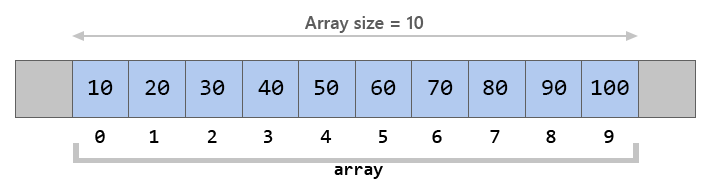
\includegraphics{array.png}
		}
		\caption{Pole a jeho indexy}
		\label{fig:Etiopanek}
\end{figure}
\end{frame}

\begin{frame}[fragile]{Pseudokód}
    \textbf{Deklarace pole o~šesti prvcích a naplnění hodnotou indexu:}
    \begin{minted}{c}
        int myArray[6];
        for(int i = 0; i < 6; i++)
            myArray[i] = i;
    \end{minted}
\end{frame}

\begin{frame}{Složitost operací}
    \textbf{Vyhledání a smazání konkrétního prvku} 
    \begin{itemize}
        \item složitost: O(n) - nutné projít (posunout) celé pole
    \end{itemize}
    \textbf{Přidání/zrušení prvku na začátku nebo na konci} 
    \begin{itemize}
        \item složitost: O(1)
    \end{itemize}
    \textbf{Nalezení nejmenšího a největšího prvku} 
    \begin{itemize}
        \item složitost: O(n)
    \end{itemize}
\end{frame}

\begin{frame}{Zdroje}
    \begin{itemize}
        \item \url{https://laptrinhx.com/remove-element-from-an-array-in-java-2026564821}
        \item \url{https://cw.fel.cvut.cz/old/\_media/courses/x33dsp/dsp-p2.pdf}
    \end{itemize}
\end{frame}
\end{document}
